% -*- mode: latex; mode: flyspell; ispell-local-dictionary: "en_US"; coding: utf-8; fill-column: 80 -*-

\documentclass{article}

\usepackage[utf8]{inputenc}
\usepackage[english]{babel}

\usepackage{amsmath,amsfonts,amssymb}
\usepackage{fullpage}
\usepackage{verbatim}

\usepackage{tikz,pgfplots}

\pgfplotsset{
  width=150mm,height=100mm,
  major grid style={thin,dotted,color=black!50},
  minor grid style={thin,dotted,color=black!50},
  grid,
  every axis/.append style={
    line width=0.5pt,
    tick style={
      line cap=round,
      thin,
      major tick length=4pt,
      minor tick length=2pt,
    },
  },
  legend cell align=left,
  legend pos=north west,
}

%%%%%%%%%%%%%%%%%%%%%%%%%%%%%%%%%%%%%%%%%%%%%%%%%%%%%%%%%%%%%%%%%%%%%%%%%%%%%%%%

\begin{document}

\title{Laufzeit binäre Suche vs. Mphf-Hashmap}
\author{Tim Tannert}
\maketitle

% IMPORT-DATA stats output/mphf_vs_bs.txt



\begin{center}
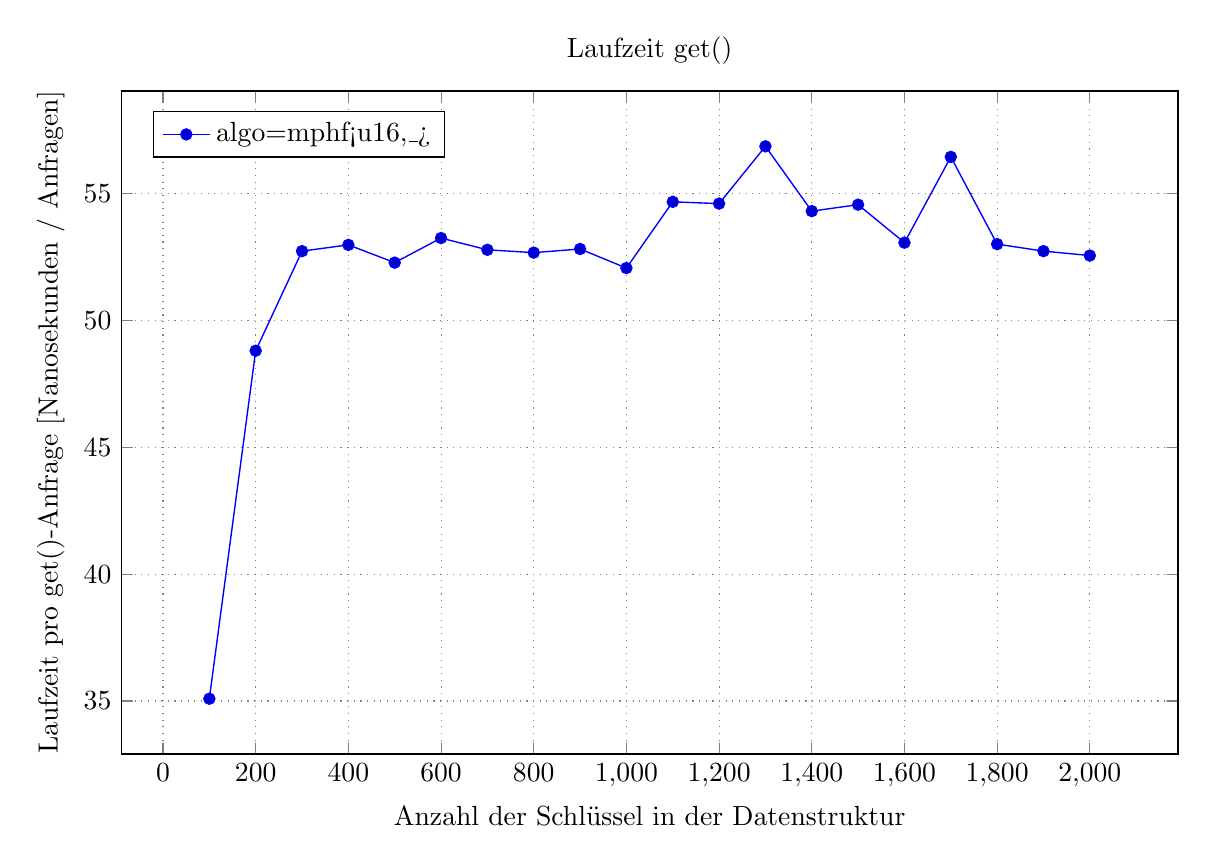
\begin{tikzpicture}
  \begin{axis}[
    title={Laufzeit get()},
    xlabel={Anzahl der Schlüssel in der Datenstruktur},
    ylabel={Laufzeit pro get()-Anfrage [Nanosekunden / Anfragen]},
    ]

    %% MULTIPLOT(algo) SELECT size AS x, MEDIAN(time_per_anfrage) AS y, MULTIPLOT
    %% FROM stats WHERE x % 100 == 0  GROUP BY MULTIPLOT,x ORDER BY MULTIPLOT,x
    \addplot coordinates { (100,35.09) (200,48.81) (300,52.7367) (400,52.9825) (500,52.283) (600,53.2517) (700,52.7879) (800,52.6769) (900,52.8206) (1000,52.069) (1100,54.68) (1200,54.6096) (1300,56.8681) (1400,54.3132) (1500,54.5673) (1600,53.07) (1700,56.4509) (1800,53.0128) (1900,52.7363) (2000,52.5615) };
    \addlegendentry{algo=mphf<u16,\_>};
    



  \end{axis}
\end{tikzpicture}
\end{center}





\end{document}
%%%%%%%%%%%%%%%%%%%%%%%%%%%%%%%%%%%%%%%%%%%%%%%%%%%%%%%%%%%%%%%%%%%%%%%%%%%%%%%%
